\documentclass{mscs}
\usepackage[pdftex]{graphicx}
\usepackage{amsmath, amsfonts}
\usepackage{listings}
\usepackage{xcolor}
\usepackage{url}
\usepackage{hyperref}
\newcommand{\Coq}{{\sc Coq}}
\newcommand{\ssr}{{\sc SSReflect}}
\newcommand{\C}[1]{\mbox{\lstinline`#1`}}
\newcommand\N[1]{\langle\mbox{\itshape\rmfamily\small #1}\rangle}
\newcommand{\iitem}{{\it i-item}}
\newcommand{\ditem}{{\it d-item}}
\let\L=\lstinline

\definecolor{dkblue}{rgb}{0,0.1,0.5} 
\definecolor{lightblue}{rgb}{0,0.5,0.5} 
\definecolor{dkgreen}{rgb}{0,0.4,0} 
\definecolor{dk2green}{rgb}{0.4,0,0} 
\definecolor{dkviolet}{rgb}{0.6,0,0.8}
\definecolor{shadethmcolor}{rgb}{0.9, 0.9,1}


\def\lstlanguagefiles{defManSSR.tex}
\lstset{language=SSR}

\lstset{moredelim=[is][\color{red}\bfseries\ttfamily\underbar]{|*}{*|}}
%Highlights metalevel expressions in italic rm font
\lstset{moredelim=*[is][\itshape\rmfamily]{/*}{*/}}



\begin{document}
\title{A formal study of Bernstein coefficients and polynomials}
\author[Y. Bertot, F. Guilhot and A. Mahboubi]{Yves Bertot,
  Fr\'ed\'erique Guilhot and Assia
  Mahboubi\thanks{This work has been partially funded by the FORMATH
    project, nr. 243847, of the FET program within the 7th Framework
    program of the European Commission and by the Galapagos project, of the
    French ANR.
}}


\newtheorem{lemma}{Lemma}[section]
\newtheorem{definition}{Definition}[section]
\newtheorem{theorem}{Theorem}[section]

\maketitle

\section{Introduction}
Bernstein coefficients provide a discrete approximation of polynomials
inside a bounded interval. As such they are useful tools to solve
problems like locating the roots of polynomials, isolating these roots
or solving systems of inequations with polynomial members.  In
computer aided design, they are also used intensively as they give an
efficient tool to draw curves that are controlled by points that users
can grab and drag, with instantaneous and intuitive feedback on the
curve's shape.  
Bernstein coefficients are closely related to B\'ezier curves
and they have a very simple geometrical interpretation, which we illustrate
in section \ref{sec:geometrybernstein}.

Bernstein coefficients are defined for a given polynomial, a given
degree, and a given interval. If the degree is \(n\), then
the coefficients form a sequence of size \(n+1\). In
this paper, we are interested in three important properties of these
coefficients:
\begin{enumerate}
\item if the coefficients taken in order exhibit exactly one sign change,
  then the polynomial is guaranteed to have exactly one root inside
  the interval.
\item  if all coefficients have the same sign, then the
  polynomial is guaranteed to have no root inside the interval.
\item there is an easy method to compute new Bernstein coefficients when
 splitting the interval in two.
\end{enumerate}

We describe a formal proof of these three properties,
concentrating on the first and third property.

The main plan of the proof of the first property is to describe a
sequence of pairs \((I_0, p_0)\) to \((I_3, p_3)\), each pair
containing an interval and a polynomial, such that every root of
polynomial \(p_i\) inside \(I_i\) is in bijective correspondence with
a root of polynomial \(p_{i+1}\) in the interval \(I_{i+1}\).  If we
study the roots of the polynomial $p$ on the interval $(l, r)$,
then $I_0$ and $p_0$ are respectively $(l, r)$ and $p$.
The last interval $I_3$ is \((0, +\infty)\) and the last polynomial
$p_3$ is \(c_0 + c_1 X + \cdots + c_n X^n\), where the coefficients
\(c_i\) have the
same sign as the Bernstein coefficients.  Going from \(p_i\) to
\(p_{i+1}\) we apply a given transformation.  The first transformation
is a change of variable such that \(I_1\) is \((0,1)\) and \(p_1(x) =
p_0(r x + l (1 - x))\).  The second transformation is such that
\(I_2\) is \((1,+\infty)\) and \(p_2(x) = 0\) exactly when \(p_1(1/x)
= 0\), as long as \(x\neq 0\).  The third transformation is a
translation such that \(I_3 = (0,+\infty)\) and \(p_3(x) = p_2(1+x)\).
We will show that the condition on Bernstein coefficients simply
boils down to Descartes' law of sign \cite{descartes, bpr} for
polynomial \(p_3\) in the
case where there is exactly one sign change in this polynomial's coefficients.
This path from one polynomial to another is described in section~\ref{sec:Bernstein}.

Descartes' law of signs provides a sufficient criterion for the
existence of exactly one root for a polynomial
between 0 and \(+\infty\).  In its
most general form, this law
expresses a relation between the number of roots of a polynomial
between 0 and \(+\infty\) and the number of sign changes in the
coefficients of this polynomial.  The number of sign changes is larger
than the number of roots and the difference between the two numbers is
even.  Thus, if the number of sign changes is 1, there is
exactly one root between 0 and \(+\infty\).

For our development, we only prove the corollary  of
Descartes' law of signs for the case where there is only one sign
change.    This proof is done in section~\ref{sec:descartes}.
  Expressing Descartes' law on the coefficients of polynomial
\(p_3\) yields directly a law expressed in terms of sign changes for
Bernstein's coefficients of \(p\) with respect to the
interval
\((l,r)\).

Another part of our work is to describe dichotomy.  Knowing Bernstein
coefficients for a polynomial and a given interval, it is easy to
obtain the Bernstein coefficients for the two half intervals, using
an algorithm due to de Casteljau \cite{castel}.  In the process, we increase
the precision of the approximation given by the Bernstein
coefficients.  De Casteljau's algorithm is a simple combinatorial
algorithm based on taking arithmetic means of successive coefficients.
To justify this combinatorial process we show in
section~\ref{sec:bernsteindef} that Bernstein
coefficients actually are the coefficients of the polynomial in a
different basis from the usual monomials, called the {\em Bernstein basis}.

In the following, we will assume that we are working with polynomials 
whose roots are all simple, called {\em separable polynomials}.
Starting from an arbitrary polynomial it is easy to produce a 
separable polynomial with the same roots by computing the greatest 
common divisor of this polynomial and its derivative.
 
All these results deal with polynomial functions over real numbers. In
order to make this formal study as generic as possible, we abstract
from the choice of the subset of real numbers of interest for the
user and only rely on an abstract structure of archimedean field. We
however require this field to be equipped with a decidable comparison:
the process we describe can in turn effectively be used in a decision
procedure.

If the field we work in is only guaranteed to be ordered and archimedean,
the existence of roots takes a
different meaning: if a polynomial has a single simple real root in an
interval, this root may not belong to the field of its coefficients. 
However, we can use a corresponding property which can be expressed in
the field of coefficients: there exists a
sub-interval inside which the absolute value of the slope is bounded
below, and such that the values of the polynomial at the sub-interval
bounds have opposite signs.  In a similar vein, the intermediate value
theorem  does not hold within the language we have chosen, but a
corresponding statement, expressed as a bounded-value property, does.
Our proof development relies on this approach.  We describe the formal
aspects of this approach to describing roots in
section~\ref{sec:rational}.

The formal work described in this paper has been performed using
the \Coq{} system \cite{coqart, coqsite}, with the \ssr{} extension
\cite{GONTHIER:2008:INRIA-00258384:4}.  We think some characteristics
of the proof system played a key role in making this development
possible.  We describe these key aspects in section~\ref{sec:formal}.
The sources of this development are available from\\
{\url{http://hal.inria.fr/inria-00503017/}}

\section{Formalization viewpoints}
\label{sec:rational}

\subsection{A constructive and abstract approach}
Our aim is to provide a constructive and effective formalization of
the theory of Bernstein polynomials, and to be as independent as
possible from the implementation choices of rational numbers and
real numbers. For this
purpose, we eliminate real points from the formalization. 
We consider polynomials with coefficients in an abstract ordered and
archimedean field. The axioms of this structure are the ones of a
field with decidable equality, with a decidable order relation which is
compatible with the field operations. The decidability of the equality
and order relations are crucial for the algorithms we describe to be
truely effective. Such a field necessarily contains a copy of rational
numbers, which are the carrier of the computations performed in our
proofs. We do not provide
nor rely on a general theory of continuous functions but rather prove
that such polynomials are necessarily continuous (and even uniformly
continuous on bounded intervals) using $\epsilon$-$\delta$ statements
quantified on elements of the coefficient field.

Since such an archimedean field has no reason
to be algebraically closed, the roots of the polynomials are not
necessarily elements of this type. We hence need to adjust the
definition of {\em root of a polynomial}. In particular, we provide a
weak version of the intermediate value theorem for polynomials, which
results in a sufficient criterion for the existence of a single real root in
an interval, expressed in the language of decidable, ordered
archimedean fields. This field of coefficients cannot be directly
instantiated by constructive reals since their comparison is not
decidable, but this was not our purpose since our weak intermediate
value theorem is only there to support the further study of Bernstein
polynomials, which have rational coefficients. If coefficients are
indeed instantiated by any implementation of
rational numbers, for instance the one embedded in some implementation
of constructive numbers, then the conclusion of the intermediate
value theorem is sufficient to implement the modulus of convergence of
a Cauchy sequence, which will be the constructive root of the
polynomial. Of course, this work is readily usable  with the
``classical real numbers'' of the standard \Coq{} library, but it also
complies with the constructive libraries also implemented in the \Coq{}
system like \cite{DBLP:conf/mkm/Cruz-FilipeGW04, russellreals,
  russellcoqreals}.

% The criteria we have chosen to describe the existence of roots are
% not faithful to the usual notion of having a root.  For instance, they
% are not satisfied by the polynomials \(x^4- x^2 + \frac{1}{4}\) and
% \(x^3-\frac{3}{2} x^2 +\frac{3}{4} x -\frac{1}{8}\), which both would
% be thought of as having roots inside \((0,1)\) in the usual sense, these
% root being respectively \(\frac{1}{\sqrt{2}}\) and \(\frac{1}{2}\).
% The curve of the first polynomial only touches the x-axis in a place that is
% not a rational number, but stays on the positive side.  The curve of
% the second one really crosses the x-axis, moreover it does so in a
% rational number.  The problem is that in both case the root is multiple
% and the slope does not satisfy the property of staying away from 0.
% This shows that the trick we used to represent roots are specially
% designed for polynomials with only simple roots and should probably not
% be used in other settings.

\subsection{Small scale reflection libraries}
This work is based on the \ssr{} libraries \cite{ssrsite}
developed with the \ssr{} extension
\cite{GONTHIER:2008:INRIA-00258384:4} of the \Coq{} system.
These libraries cover basic theories (sequences, natural
numbers, finite types, finite sets), infrastructure for notations and
theory sharing (containers, iterated operators, algebraic
hierarchies), and elementary algebra and arithmetics. 
They are developed following the path leading to a complete formal
proof of a historical result in finite group theory (namely the Odd Order
Theorem), to demonstrate that a well
understood art of formalization leads to modular, reusable formal
libraries. This work addresses theories that
are not on this path, it hence challenges the reusability of the
distributed libraries and demonstrates that they can indeed be reused
and extended.

One of the main characteristics of the methodology deployed in these
libraries is small scale reflection 
\cite{ssr-tutorial}, a proof methodology which is based on the
pervasive use of computations with symbolic symbols. 
As a consequence, predicates are formalized as often as possible as
boolean functions and a set of specialized tactics
allows the user to reason on how these functions compute.
For instance, it provides powerful automation for propositional
reasoning: in this framework, reasoning in the intutionistically
classical fragment of the \Coq{} logic is almost as convenient as it
could be in a fully classical system.
Boolean representations play a role that goes beyond automation.
They also affect the manipulation of dependent
types, especially dependent pairs (also called
$\Sigma$-types). The \ssr{} library on polynomials
illustrate this fact as described in section \ref{ssec:polys}.

\subsection{Representation of polynomials}\label{ssec:polys}
In \ssr{} libraries 
polynomials are represented by a big endian list of coefficients in
the monomial basis. A polynomial function can easily be defined from
such a list through the Horner evaluation scheme.
A bare list of coefficients would however not
provide a canonical representation since the same
polynomial can be represented by an infinite number of coefficient
lists, only differing by the number of tail zeroes. The actual
definition is the following one:
\begin{lstlisting}
Record |*polynomial*| R :=
  Polynomial {polyseq :> seq R; _ : last 1 polyseq != 0}.
\end{lstlisting}
A polynomial is hence
represented by a dependent pair consisting of a list \C{polyseq} of
type \C{(seq R)} and a
proof that the last element of this list is non zero (this proof is
not given a name, hence the use of the character {\tt \_}). The type
\C{(polynomial R)} is used with the notation \L+{poly R}+. The
parameter \C{R} is the type of the coefficients. It should in fact
be equipped with a ring structure, which provides the zero element
used in the test of the proof component.

The constant zero polynomial is represented by the empty list. A
constant non zero polynomial is represented by a list with a single
element. The monomial $X$ is represented
by the list $[0, 1]$, where $1$ and $0$ are the one and zero
constants of the underlying coefficient ring.
More generally, a non zero polynomial of degree $n+1$ is
represented by a list with $n+1$ elements. The \C{:>} symbol indicates
that the \C{polyseq} constructor is declared as a coercion: a
polynomial can at any time be seen as a list of coefficients,
forgetting about the proof that it is in normal form.

In this representation, comparing two polynomials seems to
amount to comparing component-wise two dependent pairs: the first
components of
the two pairs being the actual polynomials, and the second components
of the pairs being the proofs that they are in normal form.  The calculus of
inductive constructions underlying the \Coq{} system is not proof
irrelevant: two proofs of the same statements are not equal in
general. Hence a naive design of these polynomials as dependent pairs
would lead to an uncomfortable situation where two equal lists of
coefficients would not necessarily give two equal polynomials because
they would be associated with two different proofs of normalization. Yet if
proof irrelevance does not hold in general, two proofs of the same
boolean equality are nonetheless provably equal in the calculus of
inductive constructions without axiom.  This is known as {\em boolean
  proof irrelevance}.

If the type \C{R} of coefficients is equipped with a
boolean equality test, the second component of polynomials becomes a
proof that a certain boolean is equal to the boolean \C{true}, and
hence a proof of a boolean equality. Comparing two polynomials now
boils down to comparing only their first component, and the equality
of the proof components is given by boolean proof irrelevance.
This kind of proof irrelevant dependent pairs is widely used in \ssr{}
libraries, which therefore provide a generic infrastructure to
manipulate comparisons of their inhabitants. Moreover, again thanks
to the infrastructure of \ssr{} libraries, polynomials
canonically inherit from the boolean comparison available on
coefficients, lifted to the element-wise comparison of lists.


\subsection{Criteria for the existence of a unique root}
\label{sec:criteria}
We concentrate on a sufficient criterion for the existence of a root
inside an interval.  % This criterion is strong enough to build a Cauchy
% sequence (and its modulus of convergence) whose limit in the real numbers
% would be the root.
Our criterion is based on slopes.

Ensuring that the slope is positive or negative in some interval helps
making sure that there are not more than one root in this interval.  In our
setting, where the polynomials we consider only have simple roots, we
have the stronger
property that the slope is separated from 0 by a given ratio.  In the
case of positive slopes, we write the slope requirement for a
polynomial \(p\) inside a given interval \(I\) as follows:
\begin{definition}[Slope requirement (positive case)]
A polynomial $p$ satisfies the positive slope requirement if:
\[\exists k, (0 < k \quad \wedge \quad \forall x\ y, [x \in I \wedge y \in I
\wedge x < y \Rightarrow k(y - x) < p(y) - p (x)]) \]
\end{definition}
We also define the analogous requirement for negative slopes.

Depending on the kind of interval that we will consider, we will use
two different sufficient conditions to express the existence of a
single root in the interval.

\begin{enumerate}
\item If the interval is bounded, we express that the interval can be
  decomposed into three parts, the first part \(I_1\) where the polynomial's
  value is always negative (resp. positive),
  the second part \(I_2\) where the polynomial's
  value goes from negative to positive (resp. from positive to
  negative) with a requirement on the
  slope, and the third
  part \(I_3\) where the polynomial's value is always
  positive (resp. negative).  This is illustrated in Figure~\ref{bounded_decompose}).
\begin{figure}[h]
\begin{center}
\includegraphics[clip=true,trim= 2cm 7cm 0cm 9cm,scale=0.3]{bounded_decompose.pdf}
\end{center}
\caption{\label{bounded_decompose} A sufficient criterion for the existence of a single root in a bounded interval}
\end{figure}
\item If the interval is unbounded, we express that the interval can
  be decomposed into two parts, the first part \(I_1\) where the polynomial's
  value is always negative (resp. positive), and the second part \(I_2\)
  where there is a requirement on the slope with a positive
  (resp. negative) slope.  This is illustrated in Figure~\ref{unbounded_decompose}.
\begin{figure}[h]
\begin{center}
\includegraphics[clip=true,trim=2cm 3cm 2cm 9cm, scale=0.3]{unbounded_decompose.pdf}
\end{center}
\caption{\label{unbounded_decompose} A sufficient criterion for the existence of a single root in an unbounded interval}
\end{figure}
\end{enumerate}


\subsection{Finding locations where a polynomial's value is
  arbitrarily small}
\label{ssec:civt}
In classical mathematics dealing with real closed
fields, once we know that the
polynomial takes values of opposite sign at the bounds of an interval,
we know that there is a root for this polynomial in this interval,
thanks to the {\em intermediate value theorem}. For this work, we establish
a simplified constructive, real point free, replacement of the intermediate value
theorem specialized for polynomials.  In our setting with a field that is only guaranteed to be ordered and archimedean,
we can't be sure to produce a value on which the
polynomial of interest evaluates to zero, but we are
able to produce an input for which the polynomial's absolute value is
arbitrarily close to zero. The statement we prove has the following
form:
\begin{theorem}[Weak intermediate value theorem for polynomials]
\[
\begin{array}{l}
{\forall p~x~y~\varepsilon,\quad x < y~~\wedge~~0 < \varepsilon~~\wedge~~p(x) < 0 \leq p(y)}\\
\qquad\Rightarrow [\exists x'~ y', -\varepsilon \leq p(x') < 0 \leq p(y') \leq
\varepsilon ~~\wedge~~
x \leq x' < y' \leq y]
\end{array}
\]
\end{theorem}
\begin{proof}
We again rely on reasoning about slopes. Without loss of generality,
we can assume that the two values \(x\) and \(y\) are positive. Assuming
that the polynomial $p$ has the shape \(a + X \times p_1\), we construct
another polynomial \(p_2\) whose coefficients are the absolute values of the
coefficients of \(p_1\).  This polynomial $p_2$ is increasing so its maximum
value in \([x,y]\) is reached in \(y\).   We prove that the slope
of the polynomial between any two points inside \([x,y]\) is smaller than
\(k  = p_2(y)\).  Thus, we establish that the
slope of any polynomial is bounded in absolute value on any bounded
interval.  In particular, for any \(z, t\in [x,y]\), we have
\[|p(z)-p(t)| \leq |k \times (z - t)|.\]

For a given \(\varepsilon\), because we work in an archimedean field, we can
choose an \(n\) such that \(\frac{k(y-x)}{n} < \varepsilon\)
 We then consider the
\(n+1\) values \(a_i = x + \frac{i\times (y-x)}{n}\) for \(i = 0 \dots
n\) and we solve a
discrete problem over the values \(a_i\).  We simply need to find the
largcmpest prefix \(a_0, \ldots, a_{j-1}\) such that all values \(p(a_k)\) in this
prefix are negative.  We can set \(x' =a_{j-1}\), because the next
value \(p(a_j)\) is necessarily non-negative and
\(p(a_j) - p(x') < \varepsilon\), thus \(-\varepsilon < p(x') < 0\).
In a similar way, we can set \(y'= a_j\) because \(0 \leq p(y') < \varepsilon\).
\end{proof}
Our algorithm is illustrated in Figure~\ref{ivt}. The point selected by
our algorithm is \(a_8\), even though there are more roots in the
vicinity of \(a_1\) and \(a_2\) but neither \(a_1\) nor \(a_2\) is a
point where the polynomial takes a positive value.

\begin{figure}[h]
\begin{center}
\includegraphics[scale=0.5]{ivt.pdf}
\caption{\label{ivt} Bounding a polynomial's value}
\end{center}
\end{figure}
This theorem provides a similar result to theorem 6.1.4 from
\cite{TroelstraVDalen1}, but the proof in that book relies on a more complete
description of abstract topology than we performed of our development,
where opens and their properties with respect to continuous functions
are not mentioned.  The next theorem 6.1.5 from \cite{TroelstraVDalen1} makes it
possible to construct a Cauchy sequence to a root of the continuous
function being considered.  A variant of our theorem would also make
this possible, but this was not needed for our purposes.

\section{A simple form of Descartes' law of signs}\label{sec:descartes}
One of the main results studied in this paper
is that having only one sign change in the
sequence of Bernstein coefficients for the square-free polynomial \(p\) and the
interval \((l,r)\) ensures that there is only one root of \(p\) inside
\((l,r)\).  The proof of this result relies on a similar property for
the standard coefficients of another polynomial \(q\): if there is
only one sign change in the coefficients of \(q\) then \(q\) has
only one root inside the interval \((0,+\infty)\).  In this section, we
discuss how this property is proved formally.

\subsection{A Geometrical explanation of the proof}
Let's first describe a simple graphical argument based on curves for
polynomial functions between 0 and \(+\infty\), as shown in
Figure~\ref{graph-desc}.
\begin{figure}
\begin{center}
\includegraphics[width=0.3\textwidth]{alternated2.pdf}
\end{center}
{(a) non-negative coefficients and a non-zero constant coefficient,\\
(b) non-negative coefficients and a zero constant coefficient,\\
(c) a negative constant coefficient and all others non-negative,\\
(d) one sign change and a zero constant coefficient,\\
(e) one sign change and a negative constant coefficient}

\caption{\label{graph-desc}
Classes of polynomials with or without
sign change}
\end{figure}
To describe our proof, we rely on an inductive view of polynomials
where new polynomials are built from
existing ones by multiplying them by the polynomial \(X\) and adding a
constant; this operation is known as ``Horner's scheme''.
Polynomials with one sign change and a positive leading coefficient
are obtained by starting with a positive constant, applying Horner's
scheme a certain number of times with non-negative constants, then
applying it with a negative constant, and then applying it again a certain
number of times with non-positive constants.

Polynomials with only non-negative coefficients have curves which look
like the curves (\ref{graph-desc}-a) or (\ref{graph-desc}-b) depending on whether the first
coefficient is 0, adding a positive coefficient to a polynomial of the
form (\ref{graph-desc}-a) or (\ref{graph-desc}-b) yields a polynomial of the form (\ref{graph-desc}-a), multiplying a
polynomial of the form (\ref{graph-desc}-a) or (\ref{graph-desc}-b) by the polynomial \(X\) yields a new
polynomial of the form (\ref{graph-desc}-b).  Thus, Horner's scheme with non-negative
constants keeps polynomials in the (a-b) form.  Then, when applying
Horner's scheme with a negative coefficient (thus introducing a sign
change), the multiplication by \(X\) first builds a polynomial of the
(\ref{graph-desc}-b) form, and adding a negative constant, one obtains a curve whose
shape is given by (\ref{graph-desc}-c).  From then on, multiplying a polynomial of the
form (\ref{graph-desc}-c), (\ref{graph-desc}-d), or (\ref{graph-desc}-e) by \(X\) yields a polynomial of the (\ref{graph-desc}-d) form; adding a
negative constant to a polynomial of the form (\ref{graph-desc}-d) or (\ref{graph-desc}-e) yields a
polynomial of the (\ref{graph-desc}-e) form.  Polynomials of the form (\ref{graph-desc}-d) or (\ref{graph-desc}-e)
share the following characteristic: there exists a positive value
\(x\), such that the polynomial has a negative value between 0 and
\(x\), and the slope of the curve is strictly positive above
\(x\).  Because of the slope condition, we can also find a point where
the polynomial is positive.

Let us now give a more precise proof, outlining the concepts that are
used in the formal proof.

\subsection{Lemmas for polynomials with non-negative coefficients}
Polynomials are simply encoded by their lists of coefficients, evaluating
a polynomial at a given point is done recursively following Horner's scheme,
and recognizing polynomials with only non-negative coefficients is also
done using a simple recursive function, written in the following form:
\begin{lstlisting}
  Fixpoint |*all_pos_or_zero*| (l : seq Q) : bool :=
  if l is a::tl then (0 <= a) && all_pos_or_zero tl else true.
\end{lstlisting}
The type \C{Q} refers to the ordered field
parameterizing the development, {\tt (0 <= a)} is
a boolean value, and the type constructor
{\tt seq} is a type for lists of elements in a type equipped with a
boolean equality test.

We should notice that polynomials satisfying the boolean predicate
{\tt all\_pos\_or\_zero} may contain no positive coefficients: for this
reason, we cannot guarantee that they are increasing or strictly positive
anywhere between 0 and \(+\infty\).

We prove easily by induction on lists that if they contain only non-negative
coefficients, then the corresponding polynomial always has a non negative value
for inputs in \((0,+\infty)\) and from then, we also prove by induction that
any polynomial with only non-negative coefficients is constant or increasing.

We then prove that for every polynomial \(p\)  with non-negative coefficients,
the product \(x \times p(x)\) can be made arbitrarily close to 0 while
$x$ stays in \((0,+\infty)\).

\subsection{Two lemmas on slopes}
A first lemma on slopes concerns the existence of points where a
polynomial \(p\) takes a value above an arbitrary bound \(a\).  If the slope
is bounded below by a positive ratio \(k\), this is guaranteed as it
suffices to take an input that is large enough.  As the proof is
constructive, we need to be more precise: assuming the slope is larger
than \(k\) for any \(y\) larger than \(x_1\), it suffices to take any
input larger than \(x_1 + \frac{a - p(x_1)}{k}\).  This result is
remembered in our development under the name \C{|*above\_slope*|}.

A second lemma on slopes concerns the slope of a product of the form
\(x \times p(x)\).  This
lemma reproduces the known formulas for the derivative of products of derivable
functions, but is expressed solely in terms of lower bounds of slopes:
 If  a function \(f\) has a slope larger than or equal to a non-negative
ratio \(k_f\) when \(x\) is larger than a certain bound \(a\), 
then the slope of the product \(x \times f(x)\) is larger than
\(a k_f + f(x)\).

This statement requires \(f\) to have a positive slope, but it leaves open
whether \(f(x)\) is positive or not.  In particular, the values \(a\) and
\(k_r\) can be fixed for a large interval: we intend \(a\) to be the lower
bound of interval \(I_2\) as used in the criterion for existence of a unique
root in an unbounded interval (see Figure~\ref{unbounded_decompose}).

\subsection{Polynomials with exactly one sign change}
We can now address the case of polynomials with exactly one sign
change.  We want
to show that these polynomials have exactly one root.  We exhibit the
two intervals described in the criterion for unbounded intervals (see
Figure~\ref{unbounded_decompose}) the positive value \(x_1\) and the
positive ratio \(k\) such that the polynomial is negative in the
interval \((0, x_1)\) and the slope between any two values above
\(x_1\) is larger than \(k\).

To detect polynomials with exactly one sign change, we use two recursive
functions.  The first one, which we call {\tt alternate\_1}, recognizes
polynomials with at least one positive coefficient, preceded by any number
of non-positive coefficients (possibly 0), and followed by only non-negative
coefficients, as checked by {\tt all\_pos\_or\_zero}.  This function is
defined as follows:
\begin{lstlisting}
Fixpoint |*alternate_1*| (l:seq Q) : bool :=
  if l is a::tl then
     if 0 < a then all_pos_or_zero tl else alternate_1 tl
  else false.
\end{lstlisting}
The second function, which we call {\tt alternate}, checks for the
presence of at least one negative coefficient and then calls {\tt alternate\_1}.

As we have two recursive functions, {\tt alternate\_1} and {\tt alternate},
we actually need to perform two proofs by induction.  Each proof by induction
shows that some invariant is satisfied.

The invariant for {\tt alternate\_1}
must be satisfied by a polynomial \(p\) that may or may not contain a negative
coefficient, so that this invariant cannot guarantee the existence of
places where the polynomial takes a negative value.  Instead, this invariant
guarantees for any positive \(\varepsilon\) the existence of a positive {\tt x}
and a \(k\) such that:
\begin{enumerate}
\item for any \(y\) between \(0\) and \(x\), \(p(y) \leq p (x)\) ,
\item the slope between two points larger than \(x\) is guaranteed to be larger
than \(k\),
\item the number \(x \times p(x)\) is between \(0\) and \(\varepsilon\).
\end{enumerate}

The invariant for {\tt alternate} is exactly the criterion we use
to describe the existence of exactly one root in an unbounded
interval as in section~\ref{sec:criteria}.
This proof by induction is done by induction on the list.  The empty list
does not satisfy the predicate {\tt alternate} so that this case is
easily taken care of.  The other case is when the polynomial is described
by a list of the form {\tt \(a\)::\(l\)}, so that \(l\) represents another polynomial
\(p_l\) and \(p(x) = a + x \times p_l(x)\).  Here another case distinction must be
studied, depending on whether \(a\) is zero or negative.

If \(a\) is negative, we cannot use an induction hypothesis, because in
this case \(l\) is only guaranteed to satisfy the predicate
{\tt alternate\_1}.  On the other hand, the invariant for {\tt alternate\_1}
guarantees the existence of an \(x\) such that \(x\times p_l(x)\) is positive
and smaller than \(-a\), this \(x\) is the right witness and the slope is
\(p_l(x)\).  Since \(p_l(y) \leq p_l(x)\) when \(y< x\) it is easy to
prove that \(a+y\times p_l(y)=p(y)\) is negative when \(0 < y \leq x\).  To reason on the slope, we use our lemma about the
slope of \(x \times p_l(x)\), using \(0\) as a lower bound for the slope of \(p_l\) (we only
know that it is increasing).

If {\tt a} is
zero, we have by induction hypothesis that there exist \(x\) and \(k\)
such that \(p_l\) is negative on the left of \(x\) and has a slope larger than
\(k\) on the right of \(x\).  However, this does not guarantee that \(x\) is
the right witness for \(p\) because the slope of \(x\times p_l(x)\) is only
larger than \(p_l(x) + x \times k\), and \(p_l(x)\) is negative.  The solution
is to note that \(p_l\) necessary takes a positive value in some point \(v_1\)
on the right of \(x\) and to use our
{\em constructive intermediate value theorem} from
section~\ref{ssec:civt} to
build a new value \(x_1\) such that \(-\frac{k v_1}{2} \leq p_l(x_1)
\leq 0\) and \(x_1 < v_1\).
Now \(p_l\) is still guaranteed to be negative between \(x\) and \(x_1\),
because of the slope condition, and the slope on the right of \(x_1\) is
guaranteed to be larger than \(\frac{k v_1}{2}\), which is positive.


\section{Bernstein polynomials, Bernstein coefficients}
\label{sec:bernsteindef}
B\'ezier curves \cite{bezier} are parametric curves that are widely used
to construct
smooth plane curves whose shapes are governed by a finite finite number
of \emph{control points}. A B\'ezier curve controlled by $n+1$ points is
a polynomial expression of degree $n$ in its parameter $t$. For
instance, given two points $P_0$ and $P_1$, the corresponding B\'ezier
curve is the segment $B_{(P_0, P1)}(t) = tP_0 + (1 - t)P_1$. For three control
points $P_0, P_1, P_2$, the B\'ezier curve is
$B_{(P_0, P_1, P_2)}(t) = (1 - t)^2P_0 + 2(1 - t)tP_1 + t^2P_2$.
We already see in this case that a B\'ezier
curve does not meet all its control points. In fact, it is only
guaranteed to pass through the first and the last control point. In
the case of the quadratic B\'ezier curve, the middle control point $P_1$
is the intersection of the tangents to the curve at $P_0$ and
$P_2$. The general formula giving the B\'ezier curve with $n+1$ control
points is:
$$B_{(P_0, \dots,P_n)}(t) = \sum_{k = 0}^n \binom{n}{k}(1 - t)^{n - k}t^k P_i$$
which satisfies the recursive relation:
$$B_{(P_0,\dots, P_n)}(t) = (1 - t)B_{(P_0, \dots, P_{n-1})}(t) + tB_{(P_1, \dots, P_n)}(t)$$

B\'ezier curves are named after the engineer Paul B\'ezier who was working
in the design division of a car manufacturing company. These curves have very interesting properties for
interpolation but also for computer graphics: a B\'ezier curve is
contained in the convex hull of its control
points and uniform transformations on the control points like
translation or rotation have the same effect on the curve. Points
control the shape of the curve since the $k$-th derivative of the
curve at its extreme points is governed by the $k+1$ nearest
control points.

Computer graphics algorithms usually use piecewise polynomial paths
(called splines) of  low degree. B\'ezier curves are often used to
build these splines, resulting in the so-called B\'ezier splines. Most
modern vector graphics standards, like for instance SVG, feature
support for B\'ezier splines.
TrueType fonts use quadratic B\'ezier
splines, whereas PostScript or MetaFont \cite{metafont} use cubic
B\'ezier splines.


Bernstein polynomials are defined as the weight assigned to each
control point: the $k$-th Bernstein polynomial $P_b(n, k)$ is defined by:
$$B_{(P_0, \dots,P_n)}(t) = \sum_{k = 0}^n P_b(n, k)(t)P_k$$
hence:
$$P_b(n,  k)(t) = \binom{n}{k}(1 -t)^{n - k}t^k$$

% For an arbitrary natural number \(n\), we can consider the set of polynomials
% of degree smaller than \(n\) as a vector space, and the monomials
% \(x^k\), with \(0 \leq k \leq n\) constitue a basis, the standard basis,
% of of this vector space.
% If \(p\) is a polynomial with coefficients \(a_i\), then
% \(p(x) = \sum_{i=0}^n a_i x^i\)  and the coefficients \(a_i\) are also the
% coefficients of \(p\) in the standard basis.

For arbitrary numbers \(l\) and
\(r\), we can also consider the following polynomials, called
the {\em Bernstein polynomials for degree \(n\) and the interval
\((l,r)\)} for \(0 \leq k \leq n\)
\[P_b(n, l, r, k) = \binom{n}{k} \frac{(x-l)^{k}(r-x)^{n - k}}{(r-l)^n}\]
These polynomials also constitute a basis of the vector space of polynomials
of degree \(n\), and we will usually call it the {\em Bernstein basis} leaving
the degree and the values \(l\) and \(r\) unspecified.
Every polynomial \(p\) of degree \(n\) hence has a sequence of coefficients
\((b_i)_{0\leq i \leq n}\), such that \(p(x) = \sum_{i=0}^n b_i P_b(n,l,r,i)(x)\).  The coefficients
\(b_i\) are the {\em Bernstein coefficients} of $p$.

When \(l < r\), the Bernstein polynomials are positive on $(l, r)$ and
each polynomial
of index \(k\) reaches its maximum at the point \(d_k=l+\frac{(r-l)k}{n}\), so
that each coefficient \(b_k\) somehow has a dominant influence on the value
of the polynomial around \(d_k\).  Moreover, the coefficients
\(\binom{n}{k}\) included in the definition of \(P_b(n,l,r,k)\) are chosen
in such a way that the $k$-th coefficient \(b_k\) of $p$ would tend to
have a value
close to the one of $p$  in \(d_k\).  For instance, if 
\(p_1\) is the constant polynomial with value \(1\), then all its Bernstein
coefficients are equal to 1; similarly, if \(p_2\) is the identity polynomial,
and \(n\) is larger than \(0\),
then the Bernstein coefficients for \(p_2\)
are \(l + \frac{(r-l) k}{n}\), as can
be verified using the following computation:
\begin{eqnarray*}
\lefteqn{\sum_{i=0}^n \left(l + \frac{(r-l)i}{n}\right) \binom{n}{i} \frac{(x-l)^i (r-x)^{n-i}}
{(r-l)^n}}\\
&=& \sum_{i=0}^n l \binom{n}{i}\frac{(x-l)^i(r-x)^{n-i}}{(r-l)^n} +
\sum_{i=0}^n \frac{i}{n}\binom{n}{i}\frac{(x-l)^i(r-x)^{n-i}}{(r-l)^{n-1}}\\
&=& l \frac{((x -l) + (r - x))^n}{(r-l)^n} +\sum_{i=1}^n \binom{n-1}{i-1}\frac{(x-l)^i(r-x)^{n-i}}{(r-l)^{n-1}}\\
&=& l +{ (x-l)\sum_{i=0}^{n-1}\binom{n-1}{i} \frac{(x-l)^i(r-x)^{(n-1)-i}}
{(r-l)^{n-1}}}\\
&=& l + (x -l) \frac{((x-l) + (r - x))^{n-1}}{(r-l)^{n-1}} = x
\end{eqnarray*}
At the first equality sign, we distribute inside the first sum; in the
second term, we simplify the denominator with the numerator \((r-l)\).
At the second equality sign, we recognize that the first term contains
a binomial formula corresponding to \(((x-l)+(r-x))^n\); in the second
term, we recognize that the first element of the sum can be removed
because it is 0, also we recognize that \(\frac{i}{n}\binom{n}{i}\) is
\(\binom{n-1}{i-1}\) when \(i\neq 0\).  At the third equality sign,
we use the equality \((x-l)+(r-x)=r-l\) for the first term and
we factor out \((x-l)\) from the remaining indexed sum and re-index that sum.
We then recognize another binomial formula and can conclude.

\label{sec:geometrybernstein}
The Bernstein coefficients are related to a broken line (made of
contiguous straightline segments) which gives a rough approximation of the
polynomial's function graph.  More precisely, given the bounds \((l,r)\)
of the interval, and the Bernstein coefficients \((b_0,\ldots, b_n)\)
of polynomial $p$, the $n+1$ points with coordinates \((l + i
\frac{r-l}{n}, b_i)\) are the control points for the B\'ezier curve
that coincides with the polynomial's graph. This is illustrated in Figure~\ref{control}.
\begin{figure}
\begin{center}
\begin{tabular}{ccc}
\includegraphics[width=.30\textwidth,clip=true, trim=2cm 4cm 1cm 6.3cm]
{control.pdf}&
\includegraphics[width=.30\textwidth,clip=true, trim=2cm 4cm 1cm 6.3cm]
{control2.pdf}&
\includegraphics[width=.30\textwidth,clip=true, trim=2cm 4cm 1cm 6.3cm]
{control3.pdf}\\
(a) 1, 3, -10, 1, 4, 1 & (b) 1, 3, -1, 1, 4, 1 & (c) 3, 0, 1, 10, -2, -1\
\end{tabular}
\end{center}
\caption{\label{control} Bernstein Control points and corresponding polynomial curves}
\end{figure}

In Figure~{(\ref{control}-a)} the illustration shows that a peak in
the disposition of the control points corresponds to an inflexion in the
polynomial's curve (the Bernstein coefficients are 1, 3, -10, 1, 4, 1
and -10 corresponds to a downward peak).  In this case, the peak
provokes two sign changes, which are reproduced in the shape of the
curve and correspond to the existence of two roots inside the
interval.  In Figure~(\ref{control}-b), the coefficients still exhibit
a downward peak with a negative coefficient, but the polynomial's
curve stays away from the x-axis and the two sign changes in the
Bernstein coefficients do not correspond to any real root for the
polynomial (this is a false alert).  In Figure~(\ref{control}-c),
there is one sign change, so that the first and last coefficients have
opposite signs.  In fact, the first and the last Bernstein
coefficients are equal to the values of the polynomial at the bounds
of the interval, so this imposes the existence of at least one root.
But because there is exactly one sign change in the coefficients, we
can be sure that any other bend in the curve stays away from the x-axis.


\section{From Bernstein to Descartes}\label{sec:Bernstein}
In this section, we clarify the polynomial transformations that link
the problem of finding the roots of a polynomial inside an arbitrary
bounded interval \((l,r)\) successively with the problem of finding
the roots of another polynomial inside the interval \((0,1)\) and
with the problem of finding the roots of yet another polynomial inside
the interval \((0,+\infty)\).  These transformations make it possible to
compute another collection of coefficients, which happen to be very simply
related to Bernstein coefficients.

\subsection{A criterion for the interval \((1,+\infty)\)}
Descartes' weak law of signs gives us a sufficient condition to
determine when the
unbounded interval \((0,+\infty)\) contains exactly one root for a
polynomial. Through a change of variable, we obtain a similar
criterion for the interval \((1, +\infty)\).

In the following, we will call \(\theta_v\) the transformation that
maps any polynomial \(p\) to the polynomial \(y \mapsto p(y+v)\).  If
\(p=\sum_{i=0}^n a_i x^i\), we have the following formula:
\[p(y+v)= \sum_{i=0}^{n} a_i (y+v)^i = \sum_{k=0}^{n}
(\sum_{i=k}^{n}a_i\binom{i}{k}v^{i-k}) y^k\]

The polynomial \(p\) has exactly one root in the interval \((v,+\infty)\)
if  and only if
the polynomial \(\theta_v(p)\) has exactly one root in the interval
\((0,+\infty)\).  % This is particularly interesting for the case where
% \(v=1\).
We proved this lemma.

Thus, if we apply Descartes's law of signs on the coefficients
\(\sum_{i=k}^{n}a_i\binom{i}{k}\)
 we
can obtain a sufficient criterion for the existence of exactly one
root of the polynomial \(p=\sum_{i=0}^{n}a_ix^i\) in the interval
\((1,+\infty)\).
\subsection{A criterion for the interval \((0,1)\)}
Descartes' law of signs works for unbounded intervals.  In this
section, we see how to cover also bounded intervals. The trick here relies
on reversing the polynomial's list of coefficients.  Obviously, the
number of sign changes in a list of coefficients is the same as the
number of sign changes in the reversed list.

However, the roots of a polynomial on the interval \((1,+\infty)\)
are in one-to-one correspondence with the roots of the
reversed polynomial in \((0,1)\). This is due to the following
equation:
\[\sum_{i=0}^{n}a_i x^i = x^n\times\sum_{i=0}^{n}a_i x^{i-n}\]
We can now perform another change of variable, here \(y=1/x\) and a
change of index \(j=n-i\) in the sum.
\[\sum_{i=0}^{n}a_i x^i = (\frac{1}{y})^n \sum_{j=0}^{n}a_{n-j} y^j\]
The polynomial \(\sum_{j=0}^{n} a_{n-j}y^j\) is exactly the reversed
polynomial in \(y\), and the expression \((\frac{1}{y})^n\) never becomes 0 for
\(y\in (0,1)\).  Thus, \(x\) is a root of the polynomial between \(1\)
and \(+\infty\) if and only if \(y=x^{-1}\) is a root of the reversed
polynomial between \(0\) and \(1\).

Let us note \(\rho\) the function that computes the reverse of a
polynomial.  Here we need to be precise: the coefficients of a
polynomial of degree \(n\) actually are the coefficients of a vector
in an \(n+1\) dimensional space, whose basis is made of the monomials
\(X^i\) where \(i\in\{0,\dots, n\}\).  Seen as an operation on this vector
space, \(\rho\) is an involutive automorphism.  But
polynomials of degree less than \(n\) are also elements of this vector
space and the reverse operation must be understood as reversing the
list of coefficients of length \(n+1\) obtained by padding the
polynomials description with enough 0 coefficients.


To illustrate the correspondence between a polynomial and its reverse,
we can consider the polynomial \(p(x) = x^2 + \frac{3}{2} x - 1\),
the reversed polynomial is \(q(x) = -x^2 + \frac{3}{2}x + 1\) and after
the variable change we obtain the polynomial \(-x^2-2x+1\)
which exhibits only one sign change.  This predicts that the polynomial has
exactly one root between 0 and 1, and indeed the two roots of the initial
polynomial are -2 and 1/2.  This is illustrated in
Figure~\ref{invert} where the curve with a solid line is the curve for the
polynomial \(p\), while the curve with a dashed line is the curve for
the polynomial \(q\), which has a single root between 1 and \(+\infty\).
\begin{figure}
\begin{center}
\includegraphics[clip=true,trim=0cm 1cm 0cm 4.5cm, width=0.25\textwidth]{invert.pdf}
\end{center}
\caption{\label{invert} Curves of \(x^2+\frac{3}{2}x-1\) (solid line)
and its reverse \(-x^2 + \frac{3}{2} x + 1\) (dashed)}
\end{figure}

As a conclusion, we can establish a correspondence between unique
roots in \((1,+\infty)\) of a polynomial \(p\) and unique roots in
\((0,1)\) of the polynomial \(\rho(p)\).  When working in a field that
is only guaranteed to be ordered and archimedean, this
correspondence works by linking the criterion for unbounded intervals
with the criterion for bounded intervals.  The proof of this
correspondence
involves the
computation of the slope for \(x^np(1/x)\) from the slope of \(p\),
which makes it trickier than other proofs of this section.  This is again a place where
our constructive intermediate value theorem plays a role.

\subsection{Handling arbitrary bounded intervals}

The next step is to relate the roots of any polynomial inside an
arbitrary interval \((l,r)\) with the roots of another
polynomial inside the interval \((0,1)\).  This is done with another
change of variable, this time \(x= (r-l) y + l\). In other words, the
polynomial function which maps any \(x\) to \(p(x)\) has a root
between \(l\) and \(r\) if and only if the polynomial function which
maps any \(y\) to \(p((r - l) y + l)\) has a root between 0 and 1.

Here again, we can define a generic transformation on polynomials,
named \(\chi_k\) that corresponds to expanding with a given ratio $k$.
For an arbitrary polynomial \(p=\sum_{i=0}^n a_i X^i\), the polynomial
\(\chi_k(p)\) is defined as follows:
\[\chi_k(p) = \sum_{i=0}^n a_i(kX^i) = \sum_{i=0}^n a_ik^i X^i\]

Thus, the change of variable to study the roots of polynomial \(p\)
is actually represented by \(\chi_{r-l}\circ \theta_l\).

The geometric effect of the polynomial transformation
is illustrated in Figure~\ref{expand-translate}, where the shape
of the curve for the polynomial \(\frac{x^3}{8} - \frac{x^2}{8} + 3
x\) inside the interval \((2,4)\) is reproduced by the shape of the
curve for the polynomial \(x^3 -\frac{5}{2}x^2-2x+\frac{3}{2}\) inside
the interval \((0,1)\).
\begin{figure}
\begin{center}
\includegraphics[clip=true,trim=4.5cm 18cm 2cm 3cm, width=0.5\textwidth]{expand-translate.pdf}
\end{center}
\caption{\label{expand-translate} 
Curves of a polynomial inside \((2,4)\) and the
  corresponding transformed polynomial inside \((0,1)\)}
\end{figure}
\subsection{Recapitulating operations}\label{ssec:ops}
In our formal development, we defined the three operations for
translating (\(\theta\)), expanding (\(\chi\)),
 and reversing the list of coefficients (\(\rho\)).  We can then
compute a sequence of coefficients by applying the transformation
\[\tau = \theta_1\circ\rho\circ \chi_{r-l}\circ \theta_{l}.\]
When the coefficients we obtain have exactly one sign change, we
know that the polynomial has exactly one root inside the interval
\((l,r)\).

By construction, each of the operation \(\theta\), \(\rho\), \(\chi\)
actually is a linear application
of the vector space of polynomials of degree less than \(n\) into itself.
The inverse of \(\theta_a\) is \(\theta_{-a}\), and this is easily proved,
so that \(\theta_a\) is always bijective.  When \(k\) is nonzero,
the inverse of \(\chi_k\) is \(\chi_{\frac{1}{k}}\), so this linear
application is also bijective.  The inverse of \(\rho\) is itself.
As a result, the whole transformation is also inversible and its inverse
is \[\tau^{-1}=\theta_{-l}\circ\chi_{\frac{1}{r-l}} \circ \rho \circ \theta_{-1}.\]
We proved that the images of the monomials \(X^i\) by this inverse
transformation are multiples of the Bernstein polynomials, in reverse order.
Let us first observe the effect of \(\rho\circ \theta_{-1}\):
\begin{eqnarray*}
\tau^{-1}(x^i)=
\theta_{-l}\circ\chi_{\frac{1}{r-l}} \circ \rho\left(\sum_{j=0}^i\binom{i}{j}(-1)^jx^{i-j}\right)
&=&
\theta_{-l}\circ\chi_{\frac{1}{r-l}}\left( \sum_{j=0}^i\binom{i}{j}(-1)^j x^{n-i+j}
\right)\\
&=&\theta_{-l}\circ\chi_{\frac{1}{r-l}}\left(x^{n-i}\sum_{j=0}^i\binom{i}{j} (-x)^j\right)\\
&=&\theta_{-l}\circ\chi_{\frac{1}{r-l}}\left(x^{n-i}(1-x)^i\right)
\end{eqnarray*}
Then let's observe the effect of \(\theta_{-l}\circ\chi_{\frac{1}{r-l}}\).
\begin{eqnarray*}
\tau^{-1}(X^i)
&=&\theta_{-l}\left(\frac{x^{n-i}}{(r-l)^{n-i}}\left(1-\frac{x}{r-l}\right)^i\right)\\
&=&\theta_{-l}\left(\frac{x^{n-i}}{(r-l)^{n-i}}\frac{(r-l-x)^i}{(r-l)^i}\right)
\\
&=&\theta_{-l}\left(\frac{x^{n-i}(r-l-x)^i}{(r-l)^n}\right)\\
&=&\frac{(x-l)^{n-i}(r-l-(x-l))^i}{(r-l)^n}\\
&=&\frac{1}{\binom{n}{i}}(P_b(n,l,r,n-i))
\end{eqnarray*}
If the transformation \(\tau(p)\) leads to a sequence
of coefficients \(c_i\), this means \(\tau(p)=\sum_{i=0}^{n} c_i x^i\).  Now,
using the fact that both \(\tau\) and \(\tau^{-1}\) are linear, we can see
that the polynomial \(p\) is
\begin{eqnarray*}
p&=&\tau^{-1}\left(\sum_{i=0}^{n} c_i X^i\right)\\
&=&\sum_{i=0}^{n}c_i\tau^{-1}(x^i)\\
&=&\sum_{i=0}^{n}c_i\frac{1}{\binom{n}{i}} P_b(n,l,r,n-i)
\end{eqnarray*}
Thus, the Bernstein coefficients are obtained in the following manner:
\[b_i=\binom{n}{n-i}^{-1}c_{n-i} = \binom{n}{i}^{-1}c_{n-i}\]
Since the number of sign changes does not depend on the order
in which the list is observed, we obtain the proof that one sign
change in the sequence of Bernstein coefficients implies the existence
of a root in the interval \((l,r)\).

\section{Dichotomy}

\label{sec:dicho}
Bernstein coefficients give precise information when they exhibit
either zero or one sign change. In the first case, we have the
guarantee that there are no roots of the considered polynomial in the
considered interval. In the second case, we have the guarantee that
there is exactly one root.

When Bernstein coefficients exhibit more than one sign change, no
conclusion can be drawn about the existence and unicity of roots in the
interval.  For instance, in Figure~(\ref{control}.b), the Bernstein
coefficients exhibit two sign changes, but there is no root inside the
interval.  When facing this kind of inconclusive information, the solution
is to refine the approximation given by the control line.

\subsection{Geometric intuition for dichotomy}
\label{ssec:dichogeom}
When cutting an interval in two halves, the number of control points is
approximately doubled, because each of the new half-intervals receives a
new sequence of \(n\) Bernstein coefficients.  As a result, the control points
are closer to each other and to the polynomial's curve and they give a more
accurate account of the curve's position with respect to the real
x-axis.  This is
illustrated in Figure~\ref{dichotomy-curve}, where the initial Bernstein
coefficients exhibit two sign changes, which are needed to account for the bend
in the first half of the interval (a positive local minimal, but expressed
by a negative Bernstein coefficient).  In the halved interval two more points
are added in the vicinity of the bend, and none of the control points have
to be negative anymore.
\begin{figure}
\begin{center}
\includegraphics[clip=true,trim=2cm 12cm 1cm 11cm,width=0.6\textwidth]{control4.pdf}
\caption{\label{dichotomy-curve}Bernstein control points for halved intervals}
\end{center}
\end{figure}

In Figure~\ref{dichotomy-curve}, the dotted line represents
the polynomial's curve, the solid line links the control points for
the largest interval, marked by round bullets (the Bernstein coefficients are
1, 3, -1, 1, 4, 1 for this interval).  The dashed line links the control points
for the two half intervals, marked by square boxes
(the Bernstein coefficients are 1, 2, 1.5, 1,
0.9375, 1.15625 for the first interval, and 1.15625, 1.375, 1.875, 2.5, 2.5,
1 for the second interval).  This figure illustrates that the control line
really gets closer to the polynomial's curve, and provides a much better
approximation of the polynomial.

The formula given in section~\ref{sec:bernsteindef} is useful to compute an
initial series of Bernstein coefficients, and the correctness of the
conditions for existence of roots based on these coefficients can be
justified using the transformation described in
section~\ref{ssec:ops}.

It may seem that computing Bernstein coefficients is a costly process.
Around 1950, while studying B\'ezier curves, De Casteljau noticed that
the coefficients for the sub intervals
were easy to compute from the coefficients for the big interval
through a simple recursive process, exploiting the recurrence relation
already given in section \ref{sec:bernsteindef}.  This suggests
another recursive algorithm, starting from a large interval that is
guaranteed to contain all the roots of a polynomial (see section~\ref{ssec:cauchy}) and splitting this
interval into smaller pieces until all roots have been isolated (see section~\ref{ssec:split}).

\subsection{Initialization}\label{ssec:cauchy}
Given an arbitrary non constant polynomial $p$ of degree
$n$, defined by $p = \sum_{i  = 0}^n a_iX^i$ it is actually  possible to bound the absolute values
of its roots by a simple constant defined from the coefficients
$a_i ({i = 0 \dots n})$, called the Cauchy bound \cite{bpr}:
\begin{theorem}[Cauchy bounds]
$$\forall x \in \mathbb{R}, p(x) = 0 \Rightarrow |x|
\leq C(p) \quad \textrm{with} \quad C(p) = \sum_{i=0}^n \frac{|a_i|}{|a_n|}$$
\end{theorem}
\begin{proof}
Let $x$ be a root of $p$. If $|x|\leq 1$, since $1 \leq C(p)$,
the inequality trivially holds. Then if $|x| > 1$, since $x$ is a root,
and $a_n \neq 0$
$$x^n = - \frac{1}{a_n}\sum_{i = 0}^{n-1}a_i x^i$$
Hence:
$$|x|^n \leq \frac{1}{|a_n|}\sum_{i = 0}^{n-1}|a_i| |x|^i \leq
\frac{1}{|a_n|}\sum_{i = 0}^{n}|a_i| |x|^i$$
by triangular inequality. Then:
$$|x| \leq \frac{1}{|a_n|}\sum_{i = 0}^{n-1}|a_i| |x|^{i - (n - 1)} \leq
\frac{1}{|a_n|}\sum_{i = 0}^{n-1}|a_i| $$
since $|x| > 1$ implies that forall $i = 0 \dots n-1$,
$|x|^{i - (n - 1)} \leq 1$. Finally since:
$$\frac{1}{|a_n|}\sum_{i = 0}^{n-1}|a_i| \leq \frac{1}{|a_n|}\sum_{i =
  0}^{n}|a_i|$$
we have $|x| \leq C(p)$.
\end{proof}

%  then by adding a non-negative constant
% on the right (otherwise the sum might be empty). Then:
% $$|x| \leq \frac{1}{|a_n|}\sum_{i = 0}^{n}|a_i| |x|^{i - n} \leq
% \frac{1}{|a_n|}\sum_{i = 0}^{n}|a_i| $$
% since $|x| > 1$ implies that forall $i = 0 \dots n$,
% $|x|^{i - n} \leq 1$.

This means that to start studying the roots of a polynomial $p$ we can
restrict the infinite real line to a bounded interval
$(- C(p), C(p))$. This justifies we can start a real root isolation
process by providing the initial interval of interest. On this first
interval, we compute Bernstein coefficients from the transformations
presented in the previous section. Then in case of more that one sign
change, we continue by invoking the splitting de Casteljau algorithm
explained in the next subsection.

\subsection{Splitting algorithm}\label{ssec:split}

Given three pairwise distinct rational numbers $l, r, m$,
there exists an efficient algorithm to deduce the two respective lists
of Bernstein coefficients of a polynomial $p$ on intervals $(l, m)$
and $(m, r)$ from the list of Bernstein coefficients of $p$ on
interval $(l, r)$.

Let \C{b} be the sequence of Bernstein coefficients of a polynomial
$p$ of degree \(n\) for an interval \((l,r)\).
Let $m$ be a number
distinct from $l$ and $r$. We pose
$\alpha = \frac{m - l}{r - l}$ and $\beta = \frac{r - m}{r - l}$. The
\C{|*de_casteljau*|} algorithm is defined recursively by:
\begin{lstlisting}
  Variables (alpha beta : Q).
  Fixpoint |*de_casteljau*| (b : nat -> Q) (n : nat) :=
    match n with
    | O => b
    | i.+1 => fun j =>
      (alpha * de_casteljau b i j + beta * de_casteljau b i j.+1)
  end.
\end{lstlisting}
where the initial sequence of coefficients \C{b} is represented by an
infinite sequence of rational numbers, for which only the first $n$
elements are relevant.  The following function gives the Bernstein
coefficients of \(p\) on the finite interval \((l,m)\).
\begin{lstlisting}
  Definition |*dicho'*| alpha beta c i :=
    de_casteljau alpha beta c i 0.
\end{lstlisting}
The following function gives the Bernstein coefficients of \(p\) on the
finite interval \((m,r)\).
\begin{lstlisting}
  Definition |*dicho*| alpha beta p c i :=
     de_casteljau alpha beta c (p - i) i.
\end{lstlisting}

Observing the function \C{|*de_casteljau*|}
more precisely, we see that the algorithm actually
proceeds by creating a succession of lines where the element at rank
\(j\) in a given line is obtained by computing a weighted sum of the two
elements at rank \(j\) and \(j+1\) on the previous line.

This process can be illustrated geometrically by a succession of broken
lines.
For the first line, we take the control line of the initial
interval.  Then, for each of the segments that compose this control line,
we cut this segment in the same proportion as the proportion in which
the interval is split between \((l,m)\) and \((m,r)\).  This gives us
a new collection of points.  We started with \(n + 1\) control points and
thus had \(n\) segments, we now have \(n\) new points, defining \(n-1\)
new segments.  We repeat this process with the new segments, until we reach
a situation where there is only one segment and we again split this
segment into two parts in proportion of \((l,m)\) and \((m,r)\).  The
last point is guaranteed to lie on the polynomial's curve.

Although we actually only use de Casteljau's algorithm when \(m\) is
the midpoint of the initial interval, it works for any relative
positions of \(l\), \(m\), and \(r\), as long as they are pairwise distinct.

The different points computed by the de Casteljau algorithm are
represented on Figure~\ref{dichobern}. The innermost points are the
control points in the two new bases, computed from the original control
points $\{B0, \dots, B5\}$.
The middle innermost control point, on the curve, belongs to the two
new lists of control points. Points $\{C0, \dots, C5\}$ are the
control points in the left half, $\{D0, \dots, D5\}$ are the control
points on the right half.
De Casteljau's algorithm is extensively used in computer  graphics for
rasterizing B{\'e}zier curves.

\begin{figure}[h]
\begin{center}
\includegraphics[width=0.6\textwidth]{dicho_bern.pdf}
\caption{\label{dichobern}Intermediate points computed by de Casteljau's
 algorithm on $[B0, B5]$}
\end{center}
\end{figure}


The aim of this section is to prove that this algorithms is
correct, i.e. that the \C{|*dicho*|} and \C{|*dicho'*|} function
indeed computes the expected Bernstein coefficients. The correctness
theorems as stated in \Coq{} are:
\begin{lstlisting}
Lemma |*dicho'_correct*| : forall (l r m : Q)(q : {poly Q})(p : nat)
(c : nat -> Q)
(alpha := (r - m) * (r - l)^-1) (beta := (m - l) * (r - l)^-1),
  m != l ->
  q = \sum_(i < p.+1)(c i) * bernp l r p i ->
  q = \sum_(j < p.+1)(dicho' alpha beta c j) * bernp l m p j.

Lemma |*dicho_correct*| : forall (l r m : Q)(q : {poly Q})(p : nat)
(c : nat -> Q)
(alpha := (r - m) * (r - l)^-1) (beta := ((m - l) * (r - l)^-1)),
  m != r ->
  q = \sum_(i < p.+1)(c i) * bernp l r p i ->
  q = \sum_(j < p.+1)(dicho alpha beta p c j) * bernp m r p j.
\end{lstlisting}
where \C{(bernp l r p i)} is the $i$-th polynomial in the Bernstein
basis of degree $p$ with parameters $l$ and $r$.
\begin{figure}[ht]
\begin{center}
\includegraphics[width=0.5\textwidth]{bern1.pdf}
\end{center}
\caption{\label{bern} Properties of de Casteljau computations}
\end{figure}


The properties of computations performed by the de Casteljau algorithm
are summarized on Figure~\ref{bern}. Starting from the input list
$b = (b_0^{(0)}\dots b_p^{(0)})$ of coefficients in the basis with
parameters $l$ and $r$, on the upper side of the triangle, it
computes the full triangle, so that in the end the two expected output
lists can be read on the two  other sides of the triangle. The list
$b' = b_0^{(0)} \dots b_0^{(j)} \dots b_0^{(p)}$ is the list of
coefficients in the basis with parameters $l$ and $m$ output by
\C{dicho'}. The list
$b'' = b_0^{(p)} \dots b_j^{(p - j)} \dots b_p^{0}$
 is the list of coefficients in the basis with parameters $m$ and $r$
 output by \C{dicho}.  The small triangle area on Figure~\ref{bern} shows which values
the computation of an arbitrary given point in the triangle relies on.
This structure is imposed by the fixpoint
 equation of the recursive definition of the de Casteljau algorithm:
\begin{lstlisting}
  de_casteljau alpha beta b n.+1 i =
  (de_casteljau alpha beta b n i) + (de_casteljau alpha beta b n i.+1)
\end{lstlisting}
which looks very similar to the recursive relation governing the
Pascal triangle.

Let us first notice that the shape of Bernstein polynomials implies
that:
\begin{lstlisting}
Lemma |*bern_swap*| :
 forall n i l r,
 (i <= n) -> r != l ->  bernp r l n i = bernp l r n (n - i).
\end{lstlisting}
This remark implies that if $b$ is the list of coefficients of the
polynomial $p$ in the Bernstein basis of degree $n$ with parameters
$l$ and $r$, then the reverse of $b$ is the list of coefficients of
the same polynomial $p$ in the Bernstein basis of degree $n$ with
parameters $r$ and $l$:

\begin{lstlisting}
Lemma |*bern_rev_coef*| : forall (n : nat)(l r : Q)(b : nat -> Q),
  \sum_(i < n.+1)(b i) * (bernp l r n i) =
  \sum_(i < n.+1)(b (n - i)) * (bernp r l n i).
\end{lstlisting}
This remark shows that the correctness of the \C{dicho'} function is
enough to get a certified computation of both Bernstein coefficient
lists.  If $b$ is the
initial list of Bernstein coefficients with parameters $l$ and $r$, then
reversing $b$ gives the  coefficients with parameters $r$ and $l$.
Applying \C{dicho'} on the reverse of $b$ using $r$, $l$, and $m$
computes the coefficients with parameters $r$ and $m$, hence reversing
this output gives the result expected for \C{dicho} on $b$ using $l$,
$r$, and $m$. Using a similar symmetry on the
\C{de_casteljau} algorithm, we in fact reduce the proof of the
\C{dicho_correct} specification to the proof of \C{dicho'_correct}.

By linearity, we can also reduce the proof of the \C{dicho'_correct}
specification to the case where the input polynomial $p$ is in fact
itself a Bernstein polynomial. This means that the input coefficient
list $b$ only contains zeros except at one position where the
coefficient is one.

Let us first compute the expected output of the \C{dicho'} function on
such a list. In other words, for any distinct rational numbers $l,
r, m$ and any $n\in \mathbb{N}$, given $i \leq n$, we want to compute
the coefficients of:
$$P_b(n, l, r, i) = \binom{n}{i} \frac{(X - l)^i(X - r)^{n -i}}
{(r - l)^n}$$ in the basis $(P_b(n, l, m, i))_{i = 0, \dots, n}$.
We pose
$\alpha = \frac{r -  m}{r - l}$ and $\beta = \frac{m - l}{r - l}$.
In the polynomials of the new basis, formal denominators are of the
form $(m - l)$. By noticing that:
$$\frac{X - l}{r-l} = \beta \frac{X - l}{m - l} \quad \textrm{and} \quad
\frac{r - X}{r - l} = \alpha\frac{X - l}{m - l} +\frac{m - X}{m - l}$$
and by using the binomial identity:
$$\binom{n}{i}\binom{n - i}{j - i}  = \binom{j}{i}\binom{n}{j}$$
we obtain that:
$$P_b(n, l, r, i) =
\sum_{j = i}^n\binom{j}{i}\alpha^{j-i}\beta^i P_b(n, l, m, j)  \quad (*)$$
Now to achieve the proof of the \C{dicho'_correct} lemma, it is
sufficient to prove that the values output by the \C{dicho'} function
coincide with the ones of $(*)$, which boils down to an induction on $i$.

\section{Formalization issues}
\label{sec:formal}

\subsection{Sequences, iterations, polynomials}\label{ssec:modularity}

One of the key features of \ssr{} libraries is that they devote a
substantial effort to infrastructure. For instance the library about
sequences contains as many operators as one would expect from a
functional language standard library: factories, access, filtering,
surgery\dots plus a comprehensive set of specifications for these
operators. For instance, to construct the subdivision used in the proof of the
weak intermediate value theorem proposed in section \ref{ssec:civt},
it is enough to use the following tactic line in the proof:
\begin{lstlisting}
pose sl := map (fun k => x + (y - x) * (k%:R / (n.+1%:R))) (iota 0 n.+2).
\end{lstlisting}
The \C{(iota 0 n.+2)} operator constructs the sequence of integers between
\C{0} and \C{n.+2}. Then the \C{map} generic list operator maps this
sequence to the desired subdivision of the interval $[x, y]$. The
infix \C{+}, \C{*} and \L+\+ operators are the generic notations
  respectively for addition, product and division in a field, here
  used for the ordered archimedean field that is a parameter to the
  development. The \L+%:R+ annotation is a postfix notation for the
embedding of
integers in any ring structure (see section \ref{ssec:algstruct}).
Now the index of the first point in this sequence where the polynomial has a
negative value is found by the following definition:
\begin{lstlisting}
pose a'_index := find (fun x => p.[x] >= 0) sl.
\end{lstlisting}
where again the \C{find} operator is a generic construction. The
theory available on \C{find} is sufficient to prove all the results
needed in the proof.

In the \ssr{} distribution, the sequence library is extended with a
library about iterated operations \cite{BGOBP:BIG08}. It
 provides a comprehensive infrastructure to work with the finite
iteration of operators equipped with some known properties like
associativity, commutativity or distributivity. Although the
definition of iteration is naturally based on a sequence, the library
includes a variety of indexing facilities. This library is
crucial in the proof of the de Casteljau algorithm presented in
section \ref{ssec:split}, both for the initialization with Cauchy
bounds and for proving the correctness of the computation, that is
that the output coefficients indeed provide a correct decomposition of
the initial polynomial on the Bernstein basis. The \L+\sum+ 
operator implicitly carries the properties that the iterated
operation is commutative, associative, and that there is a
product law which distributes over the sum. The \L+\sum_(i < n)+ notation
indicates that the iteration is performed on the sequence of integers
from \C{0} to {n.-1} (meaning the sum might be empty).
Manipulations of these expressions are treated in the generic
theory of iterated operators.

Sequences are also the core of the definition of polynomials. The
definition given in section \ref{ssec:polys} however provides little
facilities to define a polynomial extensionally, by simply providing
the values of its coefficients. This is made possible by the following
construction, and its associated notation:
\begin{lstlisting}
Notation "\poly_ ( i < n ) E" := (Poly (mkseq (fun i : nat => E) n)).
\end{lstlisting}
The expression \L+(mkseq (fun i : nat => E) n)+ builds a sequence 
containing the \C{n} first values of the function \C{E} over natural
numbers thanks to the generic \C{mkseq} operator. The variable \C{i}
is bound in the body expression \C{E}. The \C{Poly} function of type\\
\C{forall T, seq T -> {poly T}}
normalizes the sequence it takes as argument into a polynomial, so
that the tail zeroes are erased and a proof of normal form is added to
the obtained sequence. Hence the size of the (sequence contained in
the) polynomial \L{\poly_(i < n) E} is only smaller or equal to \C{n},
but is only equal to \C{n} if \C{E n.-1} is known to be non zero.
This construction is used to define the expansion and translation
introduced in section \ref{sec:Bernstein}, for instance:
\begin{lstlisting}
Definition |*expand*| (p : {poly Q})(k : Q) := 
   \poly_(i < size p)(p`_i * k ^+i).
\end{lstlisting}
where \C{Q} is the ordered archimedean field parameterizing the
development and \C{^+} is the exponentiation operation (see section
\ref{ssec:algstruct}). These
definitions are accompanied by correctness lemmas in term of
evaluation, like:
\begin{lstlisting}
Lemma |*eval_expand*| : forall p k x, (expand p k).[x] = p.[k * x].
\end{lstlisting}
where \C{p.[x]} denotes the evaluation of the polynomial \C{p}
at the point \C{x}.

The list of coefficients defining a polynomial is of course the
coefficients of the polynomial in the (countable) infinite basis of
monomials. In this development, we also need to consider polynomials
as vectors in the vector space of polynomials of degree less than a
fixed value, again with coordinates in the basis of monomials or in
Bernstein bases. More precisely we only use the fact that monomials
and Bernstein polynomials are two families of generators and not their
linear independence. Unfortunately, the linear algebra part of the
\ssr{} archive is not yet sufficiently well integrated to get this
easily from an existing infrastructure. We hence only define these
linear algebra operations at a low level: the list of coefficients
defining a polynomial is padded with zeroes when the list of
coefficient in a monomial basis of a certain degree is needed, and
conversely the list of coefficients in a monomial basis needs to be
normalized when we need to go back to the actual polynomial.
It would certainly be more elegant to use a generic library than to
rely on this ad-hoc solution.

\subsection{Algebraic structures}\label{ssec:algstruct}

This formalization is structured along the algebraic hierarchy proposed
by the \ssr{} libraries \cite{hieralg}. This hierarchy builds a graph
of algebraic structures based on types with decidable equalities and
implement inheritance and sharing or theories and notations through
the canonical structures type inference mechanism of the \Coq{}
system. We moreover base our proofs on an extension of this hierarchy
for ordered structures\cite{COHEN:2010:INRIA-00545778:1}. This extension
allowed to consider ordered unit rings and fields, which are unit
rings and fields equipped with a decidable (total) boolean order
relation which is compatible with addition and product. In the proofs
we describe here, the main algebraic structures involved are the field
of coefficients and the commutative ring structure that polynomials
inherit. This inheritance is completely automated by the
infrastructure already present in the \ssr{} libraries. However
natural numbers are not equipped with any such algebraic structure in
the \ssr{} library and their theory and notations are defined
separately. We can still use the same symbols for their algebraic
operations and ordering thanks to the scoping mechanism of the \Coq{}
system \cite{coqsite}, even if this sometimes require an explicit
scoping annotation in theorem statements.

Natural numbers are used to define the (discrete) exponentiation as
iterated
product in ring structures: if \C{x} belongs to a type equipped with a
ring structure and \C{(n : nat)} is a natural number, \C{x^+n} denotes 
\C{x} to the {n}-th power, i.e. \C{x * (x * .. (x * x)...)}.
Since at the time we write these lines
the \ssr{} libraries do not feature a formalization of integers,
exponentiation in a field structure can become artificially
technical: \C{x^-n} only denotes the inverse of \C{x^+n}, with a
(positive) natural number exponent. Yet for
this work this defect was not a severe limitation.
An other interesting operation is the iteration of the addition
operation in a ring structure: \C{x *+n} denotes \C{n} times \C{}x,
i.e., \C{x + (x + .. (x + x)...)}.  In a commutative ring structure,
the expression developing the power of a sum is hence:
\begin{lstlisting}
Lemma |*exprn_addl*| : forall x y n,
  (x + y) ^+ n = \sum_(i < n.+1) (x ^+ (n - i) * y ^+ i) *+ 'C(n, i).
\end{lstlisting}
as available in the \ssr{} library. This allows to combine
smoothly the binomial identities also available in \ssr{} with
operations in a commutative ring, as necessary in the correctness
proofs of the de Casteljau algorithm presented in section 
\ref{ssec:split}.
When the iterated element \C{x} is
in fact \C{1} the unit element of the ring, this operation defines a
generic image of the semi-ring of natural numbers in the
ring. Note that this operation need not be injective: this will only
be the case if the characterictic is zero.
This embedding is so widely used that a new notation is defined: \L+n%:R+
denotes \C{1 *+ n} in any ring structure. Remark that this expression
needs a context or an explicit cast to determine the ring in which the
natural number should be injected, i.e. the ring \C{1} is the unit of.
This injection appears in particular in the
hypothesis that the field is archimedean, which is necessary for the weak intermediate value theorem.
This hypothesis is stated as follows:
\begin{lstlisting}
Variable Q : oFieldType.
Hypothesis |*Q_arch*| : forall x:Q, 0 <= x -> {n : nat | x <= n%:R}.
\end{lstlisting}
where the \C{Variable Q} declares an ordered field structure
parameter, and the \C{|*Q_arch*|} hypothesis gives access to the
explicit value of an integer larger than a given element of the
ordered field. Again, the \ssr{} distribution lacks a library about
integers and rational numbers, the manipulation of the
embedding of rational numbers in this archimedean field is sometimes
unnecessarily tedious, though again this was not really an issue in
this development.

\subsection{Automation issues}
Sadly, a significant part of scripts is devoted to too
many atomic rewrite steps to normalize ring expressions, or prove trivial
consequences of the properties of order like transitivity or
compatibility with field operations. The \ssr{} libraries still
lack the standard automated proof producing decision procedures
available in the \Coq{}
system, like ring normalization or linear arithmetic decision. The
\ssr{} structures are indeed still not connected to these
mechanisms. The \Coq{} tactics on linear arithmetic are hardcoding the
representation of integers and coefficients and should rely on a more
abstract structure like the one of ordered field. 
In the case of the automation of ring identities, it would significantly
help the user if normalization could handle simultaneously the various
ring and semi-ring structures that can occur in an expression, like
the rings of polynomial coefficients, polynomials themselves and
possibly the semi-ring of natural numbers.
In the case of the automation of ordered arithmetic, proof steps
often involve non linear expressions, for which it is quite difficult
to get a truly generic and efficient proof producing decision
procedure. This is in fact part of the long term objectives of this
work, namely to
certify a complete decision procedure for the full first order theory
of real closed fields. Yet incomplete but lightweight tools could
probably be crafted to relieve the user from tedious steps when
possible.


\subsection{Current state of the formalization}
In this section, we recapitulate the main results described in this paper
that have a formal proof in our development.
\begin{itemize}
\item The absolute values of the real roots of a polynomial are bounded
  by the Cauchy bound, which is expressed only using the absolute
  values of the coefficients of the polynomial.
\item If a polynomial function \(p\)
has a negative value in \(x\) and a positive
value in \(y\), with \(x < y\), then for any \(\varepsilon\) one can
exhibit \(x'\) and \(y'\) such that \(-\varepsilon < p(x') < p(y') < \varepsilon\).
\item If a polynomial only has one sign change in its coefficients for the
standard monomial basis, then this polynomial has exactly one root between
\(0\) (excluded) and \(+\infty\).
\item If a polynomial only has one sign change in its Bernstein coefficients
for a given interval \((l,r)\), then this polynomial has exactly one root
between \(l\) and \(r\) (excluded).
\item The transformation that maps any polynomial to its Bernstein
  coefficients maps Bernstein polynomials to plain monomials.
\item De Casteljau's algorithm computes correctly the Bernstein coefficients
for the intervals \((l,m)\) and \((m,r)\) from the Bernstein coefficients
for the interval \((l,r)\).
\end{itemize}
This work is part of a more ambitious plan, aiming at providing an
efficient procedure
to isolate the roots of any polynomial.  It remains to develop the connections
between the various results that will constitute this procedure and its proof
of correctness. To certify an algorithmically naive version of such a
procedure, we still need to describe the procedure to reduce any
polynomial to a separable polynomial (a polynomial where all roots
have multiplicity 1).  The easy approach is to divide by the greatest common divisor
between the polynomial and its derivative. The reduction to separable
polynomials should not require too much effort considering the
libraries already available in the \ssr{} package.    We also need to describe the termination
of a procedure based on successive dichotomy.  This study of
termination might however require more substantial work.

Another issue will be to connect the correctness proof of such a
naive implementation with more realistic programs, like an
implementation of de Casteljau whose complexity would be
linear in the degree of the input, as
implemented in \cite{cadcoq} or even more optimized codes like the
ones of \cite{mourrainetal}.

\section{Conclusion}

Real root isolation methods by sign-change-based methods is a
classical topic, extensively studied (see \cite{rouillieretal} for a
review of the related litterature) after the pioneering work of
Uspensky \cite{uspensky}. Bernstein polynomials are used to provide
efficient implementations of these methods
\cite{mourrainetal, rouillieretal}.  To our knowledge, this work is
the first mechanized proof of de Casteljau's algorithm, and of the
building blocks of a real root isolation procedure. The closest work
to ours is probably the study of global optimization methods in \Coq{}
lead by Roland Zumkeller \cite{zumkellerphd}. Indeed, Bernstein
polynomial bases are also used to approximate continuous functions on a
closed domain. This last work results in an implementation in the
\Coq{} system of a tool to bound optima of multivariate continuous real
functions. Yet we could not find mention of a formalization of the
correctness proofs of this tool.

Other work concerned with roots of continuous functions often relies on
Newton's method.  This method has also be described formally using \Coq{}
and \ssr{}, although in a less constructive setting
\cite{Pasca}.  However, the applicability of the work is quite
different: the work in \cite{Pasca} applies to a wide variety of
functions of class C2 and it guarantees the unicity of a root in an
interval using strong constraints on the first and second derivative
of the function inside the interval.  It does not provide any tool for
the case when the chosen interval does not satisfy the conditions,
while our work provides a study of a dichotomy approach, but is
concerned solely with polynomials.

This work on Bernstein polynomials combines techniques coming from
analysis, algebra, and geometry. For instance, the properties of
reversing the list of coefficients of a polynomial are studied by
looking at the polynomial as a function from rational numbers to
rational numbers. Similarly, the proof of Descartes' law of signs
works by looking at functions and bounds on their values in various
intervals. On the other hand, the definition of Bernstein coefficients
relies on concepts that come from linear algebra: vector spaces,
bases, or morphisms. Last, de Casteljau's algorithm relies on geometry
with midpoints or segments. It is particularly exciting that we can
now study formally mathematical algorithms that use all these aspects
of mathematics.

This development is not made just for the beauty of it. The initial
goal is to provide one of the basic blocks required for cylindrical
algebraic decomposition \cite{bpr, cadcoq}. In the short term, we
want to complete this
into a full algorithm to isolate the roots of an arbitrary
polynomial. This involves proving the technique to reduce the
multiplicity of roots that we already described in the introduction,
initializing the search for roots with an interval large enough to
contain all the roots, programming the recursive dichotomy process,
and proving that this process always terminates.

For the proof of termination, we already know a mathematical argument,
described in \cite{bpr} under the name ``theorem of three
circles". However, this theorem uses arguments based on complex
numbers and we wish to find a more elementary proof, as we still want
to express our result using mainly rational numbers.  Our proof of the
law of signs already is more elementary than the ones found in
the literature.

In the long run, a good knowledge of Bernstein polynomials and
coefficients opens the door to a wide variety of tools that are
commonplace in computer aided design and robotics. B\'ezier curves
which are often used in drawing tools share a lot of properties with
Bernstein control points. Concerning robotics, splines and B\'ezier
curves can also be used to describe the trajectory of moving
vehicles.  Thus, this work may eventually be useful for the formal
verification of critical software in robotics.

\section{Acknowledgments} The authors whish to gratefully thank the
anonymous referees who have suggested numerous improvements both for
the formalization and for its description.

\bibliographystyle{alpha}
\bibliography{biblio}


\end{document}
%%% Local Variables:
%%% mode: latex
%%% TeX-master: t
%%% End:
